%
% john_slides.tex
% The main LaTeX file, referred to as $(MAINFILE).tex in the Makefile.
% This must be the ONLY .tex file in the main folder.

%
% Document class
\documentclass{MichiganTech}

%
% Information for title and final slides, and footers
%
% Personalize.tex
% Update this file with appropriate information

\presentationtitle{Ei mel quas nullam constituto, nam te timeam}
\presentationdate{24 April 2015}
\presentername{John D. Sanderson}
\presentertitle{TITLE}
\presenterdept{DEPARTMENT}
\presenteruniv{Michigan Technological University}
\presenteremail{john@mtu.edu}
\presenterphone{(906) 487-1885}
\presenterurl{http://mtu.edu/}
\finalslidenote{Thank you}
\finalslidecolor{ForestGreen} % This is not currently used


%
% Title slide
\titleslide

%
% Document begins
\begin{document}

\maketitle

%
% Non-title slide set up
\nontitleslidesetup

%%
% Slides begin (edit the contents below)

%
\begin{frame}{Outline}
  \vspace*{0.10in}
  \begin{reference}{4mm}{84mm}{Black}
    Michigan Tech's website:
    \href{http://www.mtu.edu}{\purl{http://www.mtu.edu}}
  \end{reference}

  \begin{itemize}
    \item Something
    \item Something
    \item Something
    \item Something
    \item Something
  \end{itemize}
\end{frame}

%
\begin{frame}{Slide title}
  \vspace*{0.10in}
  \begin{reference}{4mm}{84mm}{Black}
    \;
  \end{reference}

  \begin{beamerboxesrounded}[upper=definitionboxhead,lower=definitionboxbody,shadow=true]{lorem ipsum}
    \begin{flushleft}
      Lorem ipsum dolor sit amet, at qui viderer recusabo aliquando, dignissim
      evertitur ei his. Ignota iuvaret fabulas ei vim. Ne utinam inciderint quo.
      Pri ea congue postulant conclusionemque.
    \end{flushleft}
  \end{beamerboxesrounded}

  \pause
  \vspace*{0.10in}
  \begin{beamerboxesrounded}[upper=questionboxhead,lower=questionboxbody,shadow=true]{Discere dissentiet}
    \begin{flushleft}
      Discere dissentiet vel et, soluta nostrum epicurei ad eam, cu has aperiam
      vituperata. In prima quaeque diceret pri. Enim labores contentiones eos 
      at, duo altera denique nominavi ea, eos inani nominavi consectetuer at.
    \end{flushleft}
  \end{beamerboxesrounded}

  \pause
  \vspace*{0.10in}
  \begin{beamerboxesrounded}[upper=commandboxhead,lower=commandboxbody,shadow=true]{Commands}
    \begin{flushleft}
      \pcommand{make clean}\\
      \pcommand{make magic}
    \end{flushleft}
  \end{beamerboxesrounded}
\end{frame}

%
\begin{frame}{Slide title}
  \vspace*{0.10in}
  \begin{reference}{108mm}{12mm}{Black}
    
\includegraphics[width=0.15\textwidth]{UnknownWoman}\\
    
\includegraphics[width=0.15\textwidth]{UnknownMan}
  \end{reference}
  \begin{reference}{4mm}{82mm}{Black}
    Jill Smith (1903 -- 1992): American mathematician\\
    James Jefferson (1905 -- 1957): Canadian computer scientist
  \end{reference}

  \begin{itemize}
    \item The main item
          \begin{itemize}
            \item Sub item
            \item Sub item
            \item Sub item
          \end{itemize}
    \pause
    \item The other main item
          \begin{itemize}
            \item Sub item
            \item Sub item
            \item Sub item
          \end{itemize}
  \end{itemize}
\end{frame}

%
\begin{frame}{Slide title}
  \vspace*{0.10in}
  \begin{reference}{4mm}{84mm}{Black}
    \;
  \end{reference}

  At qui viderer recusabo aliquando, dignissim, $u_{i}^{n}$ and $u_{i}^{n-1}$,
  ei his $i$. In prima quaeque diceret pri eos inani, $u_{i}^{n+1}$,
  voluptaria cu
  \begin{equation*}
    \boxed{DodgerBlue}{u_{i}^{n+1} \,=\, 2\,u_{i}^{n} \,-\,
      u_{i}^{n-1} \,+\, 
      C^{2}\,\left( u_{i-1}^{n} \,-\, 2\,u_{i}^{n} \,+\, u_{i+1}^{n}\right)}
  \end{equation*}

  \vspace*{0.10in}
  $C \,=\, c\,(\Delta\,t/\Delta\,x)$ labores contentiones eos at 
  (\textsl{Courant numero}).

  \pause
  \vspace*{0.10in}
  Eam mazim aliquip cu recusabo pericula accommodare at mea
  facer affert nonumes qui ea,
  \boxalign{\begin{align*}
    u\left(i, t+1\right) \,=\, &\,2\,u\left(i, t\right) \,-\, \\
                               &\,u\left(i, t-1\right) \,+\, \\
                               &\,C^{2}\,\left[ u\left(i-1, t\right) \,-\, 2\,u\left(i, t\right) \,+\, u\left(i+1, t\right)\right]
  \end{align*}}
\end{frame}

%
\begin{frame}{Slide title}
  \vspace*{0.10in}
  \begin{reference}{4mm}{84mm}{Black}
    A fantastic collection of TikZ examples: 
    \href{http://texample.net}{\purl{http://texample.net}}
  \end{reference}

  \begin{figure}
    \begin{tikzpicture}[scale=0.45, every node/.style={scale=0.50}]
      \path[mindmap,concept color=Black,text=White]
      node[concept] {\begin{equation*}\sum_{i=1}^{N}\,\sum_{j=1}^{M}\,\alpha_{ij}\,\beta_{ji}\,=\,?\end{equation*}}
      [clockwise from=0]
      child[concept color=RoyalBlue!65!Black] { node[concept] {A1}
        [clockwise from=90]
        child { node[concept] {ABCD} }
        child { node[concept] {EFGH} }
        child { node[concept] {IJKL} }
      }
      child[concept color=OrangeRed!65!Black] { node[concept] {B2}
        [clockwise from=0]
        child { node[concept] {TUVWX} }
        child { node[concept] {YZABC} }
      }
      child[concept color=DarkGoldenRod!65!Black] { node[concept] {C3}
        [clockwise from=-45]
        child { node[concept] {123} }
        child { node[concept] {789} }
      }
      child[concept color=Plum!65!Black] { node[concept] {D4}
        [clockwise from=-90]
        child { node[concept] {$\alpha$} }
        child { node[concept] {$\beta\,\gamma$} }
        child { node[concept] {$\pi$} }
        child { node[concept] {$\eta$} }
      }
      child[concept color=ForestGreen!65!Black] { node[concept] {$\nabla\,\psi \,=\, \delta\,\phi$}
      }
      child[concept color=LightCoral!65!Black] { node[concept] {\begin{equation*}\int_{0}^{\infty}\,\frac{1}{x}\,dx\end{equation*}}
      } ;
    \end{tikzpicture}
  \end{figure}
\end{frame}

%
\begin{frame}{Slide title}
  \vspace*{0.10in}
  \begin{reference}{4mm}{84mm}{Black}
    A fantastic collection of TikZ examples: 
    \href{http://texample.net}{\purl{http://texample.net}}
  \end{reference}

  \begin{center}
    \begin{tikzpicture}[domain=0:4]
      \draw[very thin,color=gray] (-0.1,-1.1) grid (3.9,3.9);
      \draw[->] (-0.2,0) -- (4.2,0) node[right] {$x$};
      \draw[->] (0,-1.2) -- (0,4.2) node[above] {$f(x)$};
      \draw[color=red] plot[id=x] function{x} 
        node[right] {$x$};
      \draw[color=blue] plot[id=sin] function{sin(x)} 
        node[right] {$\sin x$};
      \draw[color=orange] plot[id=exp] function{0.05*exp(x)} 
        node[right] {$\frac{1}{20} \mathrm e^x$};
    \end{tikzpicture}
  \end{center}
\end{frame}

%
\begin{frame}{Slide title}
  \vspace*{0.10in}
  \begin{reference}{4mm}{84mm}{Black}
    A fantastic collection of TikZ examples: 
    \href{http://texample.net}{\purl{http://texample.net}}
  \end{reference}

  \begin{center}
    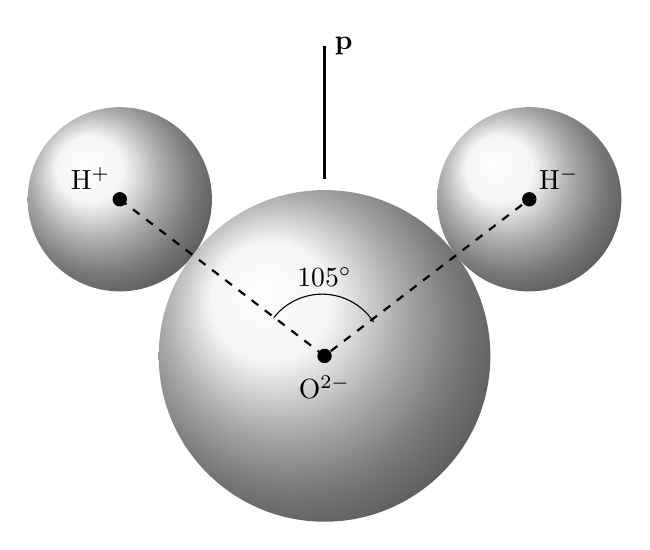
\begin{tikzpicture}[>=latex,scale=1.3]
      \shade[ball color=gray!10!] (0,0) coordinate(Hp) circle (.9) ;
      \shade[ball color=gray!10!] (2,-1.53) coordinate(O) circle (1.62) ;
      \shade[ball color=gray!10!] (4,0) coordinate(Hm) circle (.9) ;
      \draw[thick,dashed] (0,0) -- (2,-1.53) -- (4,0) ;
      \draw[thick] (2,.2) -- (2,1.5) node[right]{$\mathbf{p}$} ;
      \draw (2.48,-1.2) arc (33:142:.6)  ;
      \draw (2,-.95) node[above]{$105^{\circ}$} ;
      \draw (0,.2) node[left]{H$^+$} ;
      \draw (4,.2) node[right]{H$^-$} ;
      \draw (2,-1.63) node[below]{O$^{2-}$} ;
      \foreach \point in {O,Hp,Hm}
        \fill [black] (\point) circle (2pt) ;
    \end{tikzpicture}
  \end{center}
\end{frame}

%
\begin{frame}{Slide title}
  \vspace*{0.10in}
  \begin{reference}{4mm}{84mm}{Black}
    A fantastic collection of TikZ examples: 
    \href{http://texample.net}{\purl{http://texample.net}}
  \end{reference}

  \begin{center}
    \begin{tikzpicture}[
      thick,
      >=stealth',
      dot/.style = {
        draw,
        fill = white,
        circle,
        inner sep = 0pt,
        minimum size = 4pt
      }
      ]
      \coordinate (O) at (0,0);
      \draw[->] (-0.3,0) -- (8,0) coordinate[label = {below:$x$}] (xmax);
      \draw[->] (0,-0.3) -- (0,5) coordinate[label = {right:$f(x)$}] (ymax);
      \path[name path=x] (0.3,0.5) -- (6.7,4.7);
      \path[name path=y] plot[smooth] coordinates {(-0.3,2) (2,1.5) (4,2.8) (6,5)};
      \scope[name intersections = {of = x and y, name = i}]
        \fill[gray!20] (i-1) -- (i-2 |- i-1) -- (i-2) -- cycle;
        \draw (0.3,0.5) -- (6.7,4.7) node[pos=0.8, below right] {secant};
        \draw[red] plot[smooth] coordinates {(-0.3,2) (2,1.5) (4,2.8) (6,5)};
        \draw (i-1) node[dot, label = {above:$P$}] (i-1) {} -- node[left]
          {$f(x_0)$} (i-1 |- O) node[dot, label = {below:$x_0$}] {};
        \path (i-2) node[dot, label = {above:$Q$}] (i-2) {} -- (i-2 |- i-1)
          node[dot] (i-12) {};
        \draw (i-12) -- (i-12 |- O) node[dot,
          label = {below:$x_0 + \varepsilon$}] {};
        \draw[blue, <->] (i-2) -- node[right] {$f(x_0 + \varepsilon) - f(x_0)$}
          (i-12);
        \draw[blue, <->] (i-1) -- node[below] {$\varepsilon$} (i-12);
        \path (i-1 |- O) -- node[below] {$\varepsilon$} (i-2 |- O);
        \draw[gray] (i-2) -- (i-2 -| xmax);
        \draw[gray, <->] ([xshift = -0.5cm]i-2 -| xmax) -- node[fill = white]
          {$f(x_0 + \varepsilon)$}  ([xshift = -0.5cm]xmax);
      \endscope
    \end{tikzpicture}
  \end{center}
\end{frame}

%
\begin{frame}{Slide title}
  \vspace*{0.10in}
  \begin{reference}{4mm}{84mm}{Black}
    A fantastic collection of TikZ examples: 
    \href{http://texample.net}{\purl{http://texample.net}}
  \end{reference}

  \begin{center}
    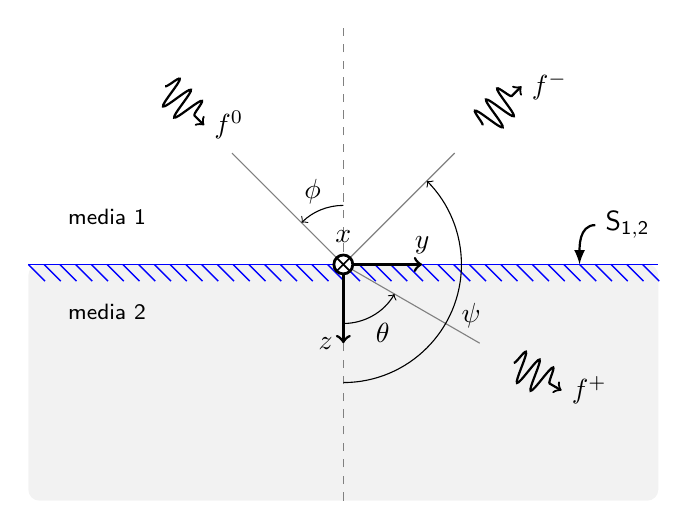
\begin{tikzpicture}[
      media/.style={font={\footnotesize\sffamily}},
      wave/.style={
        decorate,decoration={snake,post length=1.4mm,amplitude=2mm,
        segment length=2mm},thick},
      interface/.style={
        % The border decoration is a path replacing decorator. 
        % For the interface style we want to draw the original path.
        % The postaction option is therefore used to ensure that the
        % border decoration is drawn *after* the original path.
        postaction={draw,decorate,decoration={border,angle=-45,
                    amplitude=0.3cm,segment length=2mm}}},
      ]
      % Round rectangle
      \fill[gray!10,rounded corners] (-4,-3) rectangle (4,0);
      % Interface
      \draw[blue,line width=.5pt,interface](-4,0)--(4,0);
      % Vertical dashed line
      \draw[dashed,gray](0,-3)--(0,3);
      % Coordinates system
      \draw(0,0.15)node[above]{$x$};
      \draw[<->,line width=1pt] (1,0) node[above]{$y$}-|(0,-1) node[left]{$z$};
      % Incidence
      \draw[->,wave]
        (135:3.2cm)--(135:2.5cm)node[right]{$f^0$};
      \draw[gray](0:0cm)--(135:2cm);
      \path (0,0)++(113:1cm)node{$\phi$};
      \draw[->](0,0.75)arc(90:135:.75cm);
      % Transmission
      \draw[->,wave]
        (-30:2.5cm)--(-30:3.2cm)node[right]{$f^+$};
      \draw[gray](0:0cm)--(-30:2cm);
      \path (0,0)++(-60:1cm)node{$\theta$};
      \draw[->] (0,-0.75) arc (-90:-30:.75cm);
      % Reflection
      \draw[->,wave]
        (45:2.5cm)--(45:3.2cm)node[right]{$f^-$};
      \path (0,0)++(-22:1.75cm) node{$\psi$};
      \draw[gray](0:0cm)--(45:2cm);
      \draw[->] (0,-1.5)arc(-90:45:1.5cm);
      % Media names
      \path[media] (-3,.6)  node {media 1}
                   (-3,-.6) node {media 2};
      % $x$ axis
      \filldraw[fill=white,line width=1pt](0,0)circle(.12cm);
      \draw[line width=.6pt] (0,0)
        +(-135:.12cm) -- +(45:.12cm)
        +(-45:.12cm) -- +(135:.12cm);
      % Interface pointer
      \draw[-latex,thick](3.2,0.5)node[right]{$\mathsf{S_{1,2}}$}
        to[out=180,in=90] (3,0);
      % To-paths are really useful for drawing curved lines. The above
      % to path is equal to:
      %
      % \draw[-latex,thick](3.2,0.5)node[right]{$\mathsf{S_{1,2}}$}
      %      ..controls +(180:.2cm) and +(up:0.25cm) .. (3,0);
      % Internally the to path is translated to a similar bezier curve,
      % but the to path syntax hides the complexity from the user. 
    \end{tikzpicture}
  \end{center}
\end{frame}

%
\begin{frame}{Slide title}
  \vspace*{0.10in}
  \begin{reference}{4mm}{84mm}{Black}
    \;
  \end{reference}

  \begin{beamerboxesrounded}[upper=brainstormboxhead,lower=brainstormboxbody,shadow=true]{Liber liberavisse}
    \begin{flushleft}
      At vix indoctum disputando. Eam cu doctus reprimique, quaeque democritum
      an eos, sit veniam facete dissentias id. Tale volumus eos te, \pcode{P},
      an eum nulla tincidunt. Mea id recteque theophrastus, \pcode{M}.

      \vspace*{0.10in}
      Eirmod malorum vis ei. Choro euismod incorrupte in vim, ludus ornatus 
      vis ex. Hinc wisi impedit eum no, vocent definiebas referrentur in quo. 

      \vspace*{0.10in}
      \begin{equation*}
        \boxed{DodgerBlue}{S_{\mathrm{\;1}} \,=\, \frac{1}{\left(1 \,-\, P\right)\, +\, \frac{P}{M}}}
      \end{equation*}

      \vspace*{0.10in}
      \begin{equation*}
        \boxed{DodgerBlue}{S_{\mathrm{\;2}} \,=\, M \,-\, \left( 1 \,-\, P)\,(M \,-\, 1\right)}
      \end{equation*}

      \vspace*{0.10in}
    \end{flushleft}
  \end{beamerboxesrounded}
\end{frame}

%
\begin{frame}{Slide title}
  \vspace*{0.10in}
  \begin{reference}{4mm}{84mm}{Black}
    A fantastic collection of TikZ examples: 
    \href{http://texample.net}{\purl{http://texample.net}}
  \end{reference}

  \vspace*{0.10in}
  \centering
  \tikzstyle{garrow} = [draw, latex'-latex']

  \begin{tikzpicture}
    \node (proc0) [draw=none, fill=LightSteelBlue, circle, align=center, inner sep=1.5ex, minimum size=0.50in, font=\sffamily] at (0.00,0.00) {\tiny P0};
    %
    \node (proc1) [draw=none, fill=GreenYellow!90!Black, circle, align=center, inner sep=1.5ex, minimum size=0.50in, font=\sffamily] at (-4.50,-3.00) {\tiny P1};
    %
    \node (proc2) [draw=none, fill=OrangeRed, circle, align=center, inner sep=1.5ex, minimum size=0.50in, font=\sffamily] at (-1.50,-3.00) {\tiny P2};
    %
    \node (proc3) [draw=none, fill=GoldenRod, circle, align=center, inner sep=1.5ex, minimum size=0.50in, font=\sffamily] at (1.50,-3.00) {\tiny P3};
    %
    \node (proc4) [draw=none, fill=DarkMagenta!30, circle, align=center, inner sep=1.5ex, minimum size=0.50in, font=\sffamily] at (4.50,-3.00) {\tiny P4};
    %
    \path [garrow] (proc1.north) -- (proc0.south);
    \path [garrow] (proc2.north) -- (proc0.south);
    \path [garrow] (proc3.north) -- (proc0.south);
    \path [garrow] (proc4.north) -- (proc0.south);
    %
    \path [garrow] (proc1.east)  -- (proc2.west);
    \path [garrow] (proc2.east)  -- (proc3.west);
    \path [garrow] (proc3.east)  -- (proc4.west);
  \end{tikzpicture}
\end{frame}

%
\begin{frame}{Slide title}
  \vspace*{0.10in}
  \begin{reference}{4mm}{84mm}{Black}
    A fantastic collection of TikZ examples: 
    \href{http://texample.net}{\purl{http://texample.net}}
  \end{reference}

  \begin{center}
    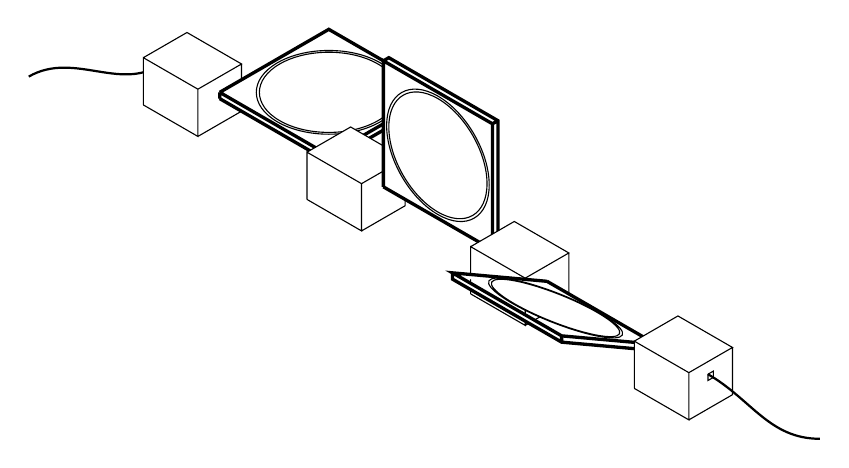
\begin{tikzpicture}[x={(0.866cm,-0.5cm)},
      y={(0.866cm,0.5cm)}, z={(0cm,1cm)}, scale=0.80]
      \tikzstyle{paddle}=[very thick, fill=white]
      \coordinate (O) at (0, 0, 0);

      % fiber in
      \draw[thick] (0,-1.5,0) to[out=30,in=220] (1,0,0);

      % first divider
      \draw[fill=white] (1,-.4,-.5) -- (2,-.4,-.5) -- (2,-.4,.25) --
        (1,-.4,.25) -- (1,-.4,-.5)
        (2,-.4,.25) -- (2,.4,.25) -- (1,.4,.25) -- (1,-.4,.25)
        (2,.4,.25) -- (2,.4,-.5) -- (2,-.4,-.5);

      % first paddle
      \draw[paddle] 
        (2,0,0) -- (4,0,0) -- (4,2,0) -- (2,2,0) -- (2,0,0) % first face
        (2,0,0) -- (2,0,-.1)
        (4,0,0) -- (4,0,-.1)
        (2,0,-.1) -- (4,0,-.1) -- (4,2,-.1);
      \draw (3,1,0) circle (.94)
        (3,1,0) circle (.9);

      % second divider
      \draw[fill=white] (4,-.4,-.5) -- (5,-.4,-.5) -- (5,-.4,.25) -- 
        (4,-.4,.25) -- (4,-.4,-.5)
        (5,-.4,.25) -- (5,.4,.25) -- (4,.4,.25) -- (4,-.4,.25)
        (5,.4,.25) -- (5,.4,-.5) -- (5,-.4,-.5);

      % second paddle
      \filldraw[paddle]
        (5,0,0) -- (7,0,0) -- (7,0,2) -- (5,0,2) -- (5,0,0) % first face
        (7,0,0) -- (7,.1,0) -- (7,.1,2) -- (5,.1,2) -- (5,0,2)
        (7,.1,2) -- (7,0,2);

      % third divider
      \draw[fill=white] (7,-.4,-.5) -- (8,-.4,-.5) -- (8,-.4,.25) --
        (7,-.4,.25) -- (7,-.4,-.5)
        (8,-.4,.25) -- (8,.4,.25) -- (7,.4,.25) -- (7,-.4,.25)
        (8,.4,.25) -- (8,.4,-.5) -- (8,-.4,-.5);

      % third paddle
      \filldraw[paddle] 
        (8,0,0) -- (10,0,0) -- (10, -1.732,1) -- (8,-1.732,1) -- (8,0,0)
        (8,-1.732,1) -- (8,-1.732,.9) -- (10,-1.732,.9) -- (10,0,-.1) -- (10,0,0)
        (10,-1.732,.9) -- (10,-1.732,1);

      % fourth divider  
      \draw[fill=white] (10,-.4,-.5) -- (11,-.4,-.5) -- (11,-.4,.25) --
        (10,-.4,.25) -- (10,-.4,-.5)
        (11,-.4,.25) -- (11,.4,.25) -- (10,.4,.25) -- (10,-.4,.25)
        (11,.4,.25) -- (11,.4,-.5) -- (11,-.4,-.5);

      \begin{scope}[x={(0.866cm,-0.5cm)},y={(0,1cm)}]
        \draw (6,0,1) circle (.94)
              (6,0,1) circle (.9);
      \end{scope}
      \begin{scope}[x={(0.866cm,-0.5cm)},y={(-.73cm,.077cm)}]
        \draw[fill=white] (9,1) circle (.94)
          (9,1) circle (.9);
      \end{scope}

      % fiber exit
      \draw (11,-.05,.05) -- (11,.05,.05) --
        (11,.05,-.05) -- (11,-.05,-.05) -- (11,-.05,.05);
      \draw[thick] (10.95,0,0) to[out=-30,in=180] (12,1,-1);
    \end{tikzpicture}
  \end{center}
\end{frame}

%
\begin{frame}{Thanks be to}
  \vspace*{0.10in}
  \begin{reference}{8mm}{75mm}{Black}
    \;
  \end{reference}

  \begin{itemize}[<+->]
    \item Someone
    \item Someone
    \item Someone
    \item Someone
    \item Someone
    \item Someone
    \item Someone
  \end{itemize}
\end{frame}

% Slides end (end of edits)
%%

%
% Final slide
\finalslide

%
% Document ends
\end{document}
